\chapter{Introduction}
\label{chap:introduction}

% intro
Software has become wide spread and integrated with mobile devices providing people with a easy to use device that can always be on them. Developers are also able to create applications which can reach a wider audience through the use of application market places such as the Google Play Store, Apple App Store. In other cases such as web development system are expected to be working constantly. The applications must provide maximum availability with minimal number of issues as possible. Developing large scale applications is a difficult task that when executed incorrectly can lead to massive losses for all parties involved in the project. 
% TODO maybe mention the number of projects that typically fail.

The software development process can be time consuming and costly even if the project is successful. During the development of a project a large number of changes will be applied to the original source code. These changes can introduce features, issues or fixes to the project. Further still, projects will often have multiple developers contributing. Managing the changes made to a project is often managed by a \gls{vcs}. A \gls{vcs} will store the change data and help facilitate the collaboration between different developers. Predicting where changes will occur within the project could help developers of a project keep track of sections of the software project that need more attention. The data may also promote a reflection on the design of the section to improve the software project.

\section{Objective \& Methodology}

% Possible reduce.
%This research is vital to improving the development process of software projects.
The mining of open source projects is widely used to help research into various software topics relating to project development and quality assurance. Research can provide improvements to the development process of software projects. With an improved development process more projects may succeed in accomplishing their outlined goal. The process of developing a project will of course take project development process will take time to complete. The time for a project to be completed relies on numerous factors including project scope, man power, experience. Over the course of project development changes will be made to project. Changes can be made to almost any part of the project including design, number of developers and type of developers. These changes will in most cases have a measurable impact on the project. In case of adding more developers the intended result may be to increase project capabilities within a shorter span of time than previously. Even with an intended result, the actual result may differ and should be measured to determine the effectiveness of a given change.

The developers of the project should manage the growth of the project to ensure that the changes that are made result in an expected outcome. Keeping track of every change to a project can be difficult because of external changes which are beyond the control of the developers. However for the majority of the changes within the project they can be kept track by using a \gls{vcs}. With proper use of a \gls{vcs} the important changes made to the project will be stored. This can help keep previous releases of the software available or even help resolve a bug that was introduced in a recent change. Furthermore, developers have control over what is stored in the \gls{vcs} allowing for granularity based on developer preferences. With numerous developers a \gls{vcs} can also help improve how these developers interact and share the changes they made. Some commonly used \gls{vcs} include Git \footnote{\url{https://git-scm.com/}}, \gls{svn}\footnote{\url{https://subversion.apache.org/}} and Mercurial\footnote{\url{https://www.mercurial-scm.org/}}.

The impact of changes can be measured and provide insights into how the project changes. However first the data must be collected, processed and stored. While changes may occur in various forms a more accessible one would be the source code changes in the software project. These changes are very fine grain since they will account for almost all functionality changes with the project. The only functionality changes not accounted by source code would be external changes (e.g. library changes). Changes will map to functionality changes that provide fixes, new functionality, or removal of functionality. The source code changes will provide a large amount of noise since every change is included. This excessive granularity can make tracking the desired changes more difficult. Visualization of the data collected allows for a more accessible look at the data to provide potential insights.


% TODO talk about project development
% - limited time
% - project costs
% - open source difference

As discussed earlier, there are two main types of projects software that are developed, either closed source or open source. \gls{oss} projects will generally provide access to the source code, the ability to change and finally redistribute the changes. \gls{oss} is widely used in developing projects of various sizes and scope. In these projects developers are able to contribute towards the a project that is often used by a wider audience. While larger \gls{oss} projects may have a small number of developers larger projects can contain developers from numerous locations around the world contributing at different times. The development of \gls{oss} is often the focus of research related to software development since the projects are open and freely available. The authors are able to publish and use the data as they wish since it is publicly available. There are also countless \gls{oss} projects to study and investigate.

The collection of data is done through data mining. Data mining is the act of collecting data from one or more sources to use for another goal. Often data mining will use a data source not traditionally used, since the goal of data mining is to extract and use information. The actual use of the data once collected can vary greatly from visualizing to modeling. Data can also be collected in several forms including continuous streams of data, sporadic data and one time collection. Depending on what type of data is being collected and the purpose of the collection the means of collection may also vary. Another concern related to data mining is that of Big Data. If a source provides a wealth of data then extra measures should be taken to manage the size of the data set. Without diligent management a data set can become unwieldy with massive overhead that are entirely avoidable.

% machine learning
The goal of the approach is to predict changes that will occur within the project using the commit history. In this case machine learning techniques are leveraged to create a model based on the data collected through mining GitHub to predict changes. Machine learning techniques are widely used to support the completion of difficult tasks that involve patterns. A machine learning algorithm is generally an algorithm that attempts to detect and mimic patterns within a data set. There are numerous different types machine learning algorithms including \gls{svm}, \gls{rf}, \gls{ann}. Each technique provides advantages and disadvantages depending on the purpose and the data set in use. The primary focus will be on \gls{svm} and \gls{rf} since they are used as part of the proposed work. In order to create the predictive model a subset from the data to be used for the training of the model. To test the model a second subset that is distinct from the first is necessary to allow measure the performance of the model.

\gls{svm} is an algorithm that attempts to classify data into two distinct categories. This algorithm is a supervised learning technique that requires a training data set to build the categorization model. The training set will consists of data samples from each classification as well as which classification the data sample belongs to. After creating the model for a \gls{svm} new data vectors can be provided to the model and be classified into one of the two categories. The model will be constructed by attempting to linearly separate the data into two distinct groups. If the data cannot be separated linearly then the data is mapped to a higher dimension to allow for proper separation. During the separation of the data points into the two groups the model may reclassify data points in an attempt to fix errors within the data set. This feature allows for some error to be present within the training set without causing further errors. In the case that points which are valid are detected as errors then the separation has generated errors and the features or data used may not be useful towards making a prediction.% TODO maybe talk about wide use of svms in research and industry?

\gls{rf} is another supervised learning technique that requires a training data set to create an prediction model. The origin of random forests is the decision tree learning method. A single decision tree creates a tree structure were each internal node in the tree represents a decision where in the final destination is the outcome. \gls{rf} extend decision trees to address the tendency for a decision tree to overfit the data. A \gls{rf} uses numerous decision trees as well as a modified version of bootstrap aggregation to get more robust predictions.

% TODO create an image of a simple decision tree

	% TODO explain svm and rf in further details.

The machine learning algorithm makes use of the training data to create a model for predicting the classification of a given value. An analysis of change data can help in the selection of useful information for creating the predictive model. The data is collected from the project's historical data that can provide a large data set to work with. Managing the data and selecting ideal samples for training must be considered to provide a strong predictive model.

\begin{figure}[!ht]
    \centering
        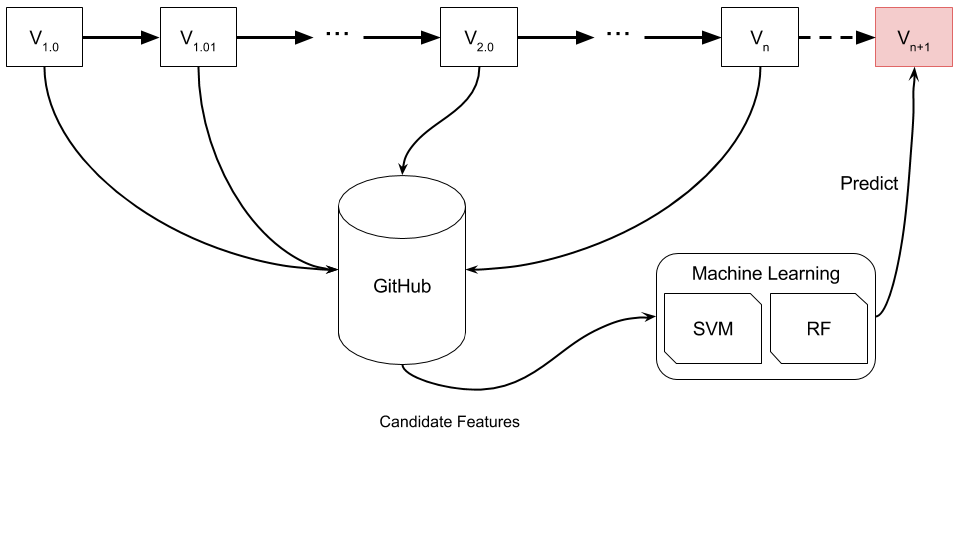
\includegraphics[width=1.0\textwidth]{images/overview}
    \caption{Approach Overview}
    \label{fig:overview}
\end{figure}

% TODO either remove or re-write this.
%This thesis generally covers topics relating to effort estimation and planning of project development. The development of a software project can vary greatly based on the scope of the project. Larger scale projects that have a complex task or set of tasks to accomplish often require a long period of time with a committed team of developers. Even once a project completely performs a task further development is needed to maintain the project for the remainder of its life.
%For the development of software in a commercial setting the ability for managers to identify the cost of a project is essential for effective business decisions. Effort estimation is one possible avenue for project managers to leverage to identify the complexity of a project and associated cost of that project. 
%The ability of developers or managers to extract more information from a project is essential to helping them make more informed decisions about the development of the project. For example if a developer can identify a location within a project that is very likely to receive changes in future development then the development may be more inclined carefully consider the types of changes necessary to make.

% TODO talk about the role of visualization?

% Thesis statement
We propose a tool that assists in managing the development of software projects by predicting changes that are likely to occur. This work explores leveraging change prediction of the source code using the commit history to assist in the development of \gls{oss} scale projects. The key factors; sampling size, feature set and data balancing are investigate using the tool to provide a deeper understanding the feasibility of the tool. Several \gls{oss} projects were selected experiment the impact of each of the factors.

\section{Contributions}

% TODO expand this section

% Contributions
Our contributions are in mining of \gls{oss}, visualization of a project's change history, machine learning change prediction, data collect which can be used and extended.

\section{Organization}
% Organization

The remainder of the this thesis is organized into 5 more chapters. \hyperref[chap:related_works]{Literature Review}, \hyperref[chap:visualization]{Visualization of Commit Data}, \hyperref[chap:prediction]{Prediction of Commit Data}, \hyperref[chap:experiments]{Experiments} and finally the \hyperref[chap:conclusions]{Conclusion}. In \autoref{chap:related_works} more details are given related to the foundation of this work. Primarily this will cover the data that is collected for the analysis. The following \autoref{chap:visualization} discusses the change visualization of the data from how the data is collected and stored. Chapter \autoref{chap:prediction} outlines the data and methods that are used for to predict change within the project. Chapter \ref{chap:experiments} reports the experiments conducted and their results. Finally the paper the conclusion summarizes the results and contributions and proposes future work to build of the thesis.